\question Draw the environment diagram that results from executing the
code below.

\begin{lstlisting}[numbers=left, numberfirstline=false]
def curry2(h):
	 def f(x):
		 def g(y):
			 return h(x, y)
		 return g
	 return f
make_adder = curry2(lambda x, y: x + y)
add_three = make_adder(3)
add_four = make_adder(4)
five = add_three(2)
\end{lstlisting}

\begin{solution}
\begin{center}
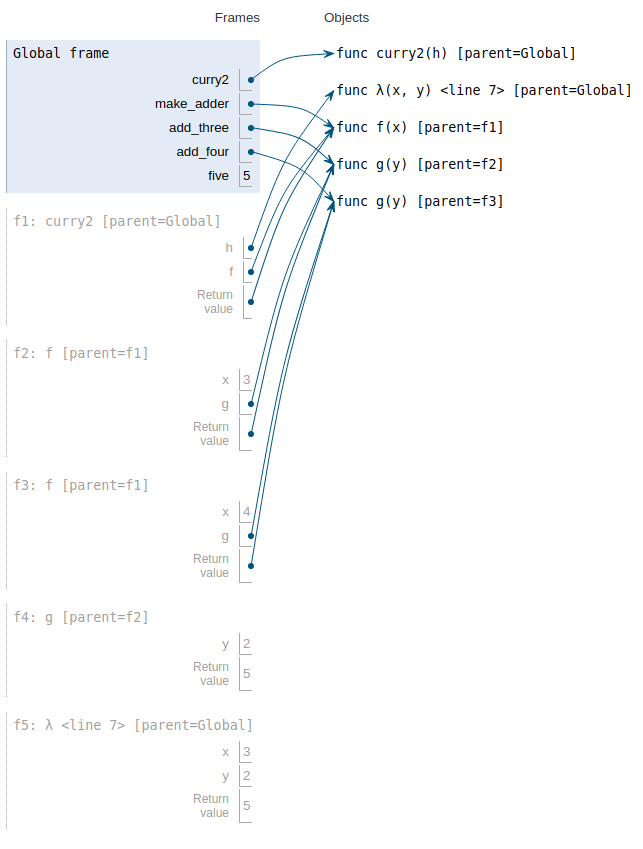
\includegraphics[width=0.7\textwidth]{curry.png}
\end{center}
\end{solution}

\newpage
\question Write \texttt{curry2} as a lambda function

\begin{solution}
\begin{lstlisting}
curry2 = lambda h: lambda x: lambda y: h(x, y)
\end{lstlisting}
\end{solution}

\bigskip
